%% --------------------------------------------------------------------
%% thesis.tex -- MAIN FILE (the one that you compile with LaTeX)
%% --------------------------------------------------------------------
%% version 1.8.09.02.16 (beta)

%-----<<<<<<<<<<<< START >>>>>>>>>>>>-----
\documentclass [a4paper,12pt]{report}  
\usepackage[a-2u]{pdfx}      		
\usepackage[cp1250]{inputenc}																	%cp1250 for Czechoslovak characters, utf8
\usepackage{lmodern}
\usepackage[T1]{fontenc}
\usepackage{textcomp}

%-----<<< --------------------------------- >>>-----

%-----<<<<<<<<<<<< DEFINITIONS >>>>>>>>>>>>----- % for special characters of Czech/Slovak lang. use LaTeX commands only such as accute accent \'{o}, caron over the letter \v{s}, etc..
\def \BookName {Master's thesis}
\def \Bookname {The Price Elasticity of Gasoline Demand: A Meta-Analysis}
\def \BooknameCZ {Cenov\'{a} Elasticita Popt\'{a}vky po Benz\'{i}nu: Meta-Anal\'{y}za} 
\def \AutorDP {Bc.\ Firstname Lastname}													
\def \AuthorDP {Firstname Lastname} 			%here use just English characters!
\def \FirstNameDP {Firstname} 				
\def \LastNameDP {Lastname} 							
\def \Email {firstname.surname@gmail.com}
\def \Year {2019}
\def \Place {Prague}
\def \Subject {Price Elasticity of Gasoline Demand}
\def \Keywords {keywordone, keywordtwo, keywordthree, keywordfour}
\def \Klic {klicjedna, klicdva, klictri, klicctyri} 					
\def \JEL {\href{http://ideas.repec.org/j/F12.html}{F12},			%http://www.aeaweb.org/journal/elclasjn_hold.html
 \href{http://ideas.repec.org/j/F21.html}{F21},								%change the codes in the argument and also in the URL
 \href{http://ideas.repec.org/j/F23.html}{F23},
 \href{http://ideas.repec.org/j/H25.html}{H25}, 	
 \href{http://ideas.repec.org/j/H71.html}{H71},
 \href{http://ideas.repec.org/j/H87.html}{H87}}	
\def \Thesisweb {\href{https://is.cuni.cz/studium/eng/dipl_st/index.php?KEY=Az1}}		%thesis webpage (leave empty if you use none)
\def \AcademicYear {2018/2019}
\def \Supervisor {prof.\ Ing.\ Willing Reader, Ph.D.}
\def \StudyProgram {Economics and Finance}
\def \EmailSup {reader@fsv.cuni.cz}
\def \CUNI {Charles University}
\def \FSS {Faculty of Social Sciences}
\def \IES {Institute of Economic Studies}
%-----<<< --------------------------------- >>>-----

%-----<<< METADATA >>>-----%filecontents must be in form of text, do not put definition reference like ``\AuthorDP'' inside
%\usepackage{filecontents}
%\begin{filecontents*}{Thesis.xmpdata}
%		\Author{Firstname Lastname} 
%		\Title{The Price Elasticity of Gasoline Demand: A Meta-Analysis}
%		\Keywords{keywordone, keywordtwo, keywordthree, keywordfour}
%		\Subject{Price Elasticity of Gasoline Demand}
%		\Publisher{Charles University} 
%\end{filecontents*} 

%-----<<<<<<<<<<<< STYLES >>>>>>>>>>>>-----      														
\usepackage{Styles/Head}
\usepackage{Styles/Mystyle}	
%-----<<< --------------------------------- >>>-----

%-----<<<<<<<<<<<< DOCUMENT >>>>>>>>>>>>-----
\begin{document}
\frontmatter                   									%lowercase roman pagination for front matter
\clubpenalty 9999 															%not so many orphants
\widowpenalty 9999 															%not so many widows

%-----<<< HEAD >>>-----
\pagestyle{empty}                       				%no visible pagination here                    
\BookHead
%-----<<< ---- >>>-----

%-----<<< DECLARATION >>>-----
\vfill

\vglue 14cm

\section*{Declaration of Authorship}
The author hereby declares that he or she compiled this thesis independently, using only the listed resources and literature, and the thesis has not been used to obtain any other academic title.

\bigskip 

\noindent The author grants to Charles University permission to reproduce and to distribute copies of this thesis in whole or in part and agrees with the thesis being used for study and scientific purposes.
\vspace{0.5cm}

\begin{table}[!hbp]
\begin{tabular}{lr}
\hspace{-0.3cm} Prague, \today
\hspace{3cm}       
 \begin{tabular}{p{4.5cm}}
    \vspace{0.6cm} \\
     \hline \\ 
		\vspace{-0.7cm} \hspace{0.6cm} \AuthorDP
 \end{tabular}

\end{tabular}
\end{table}
        					%input file
\clearpage
%-----<<< ----------- >>>-----


%-----<<< ABSTRACT >>>-----
\phantomsection													 				%bookmark anchor
\pdfbookmark[0]{Abstract}{abst}        	 				%add bookmark
\section*{Abstract}

The abstract should concisely summarize the
contents of a thesis. Since potential readers should be able to
make their decision on the personal relevance based on the abstract,
the abstract should clearly tell the reader what information
he can expect to find in the thesis. The most essential issue
is the problem statement and the actual contribution of described
work. The authors should always keep in mind that the
abstract is the most frequently read part of a thesis. It should
contain at least 70 and at most 120 words (200 when you are writing a thesis).
Do not cite anyone in the abstract.

\bigskip

\begin{tabular}{lp{8.6cm}}
		\textbf{JEL Classification} & \JEL \\
		\textbf{Keywords} & \Keywords \\
 		& \\
		\textbf{Title} & \Bookname \\
 		\textbf{Author's e-mail} & \texttt{\href{mailto:\Email}{\Email}}\\
		\textbf{Supervisor's e-mail} & \texttt{\href{mailto:\EmailSup}{\EmailSup}}\\
\end{tabular}

\bigskip

\section*{Abstrakt}\label{abstract}

TODO cesky preklad abstraktu. 

\bigskip

\begin{tabular}{lp{7.7cm}}
		\textbf{Klasifikace JEL} & \JEL \\
		\textbf{Kl\'{i}\v{c}ov\'{a} slova} & \Klic \\
 		& \\
		\textbf{N\'{a}zev pr\'{a}ce} & \BooknameCZ \\
 		\textbf{E-mail autora} & \texttt{\href{mailto:\Email}{\Email}}\\
		\textbf{E-mail vedouc\'{i}ho pr\'{a}ce} & \texttt{\href{mailto:\EmailSup}{\EmailSup}}\\
\end{tabular}

       					%input file
\clearpage
%-----<<< -------- >>>-----

%-----<<< ACKNOWLEDGMENTS >>>-----
\section*{Acknowledgments}
The author is especially grateful to PhDr. Jozef Barun\'{i}k, Ph.D., as well as Mgr. Martin Hronec for guiding, inspiring and offering valuable critics to her work both in the big picture and the technical details, always pointing to the right direction. The author is once again thankful to Mgr. Martin Hronec and his colleague MPhil. Ond\v{r}ej Tobek, Ph.D, for sharing their meticulously cleaned dataset. The author would also like to thank Bc. Tom\'{a}\v{s} Turl\'{i}k for drawing her attention to an important detail in data cleaning. A further thank you extends to RNDr. Milan Straka, Ph.D., for his outstanding courses in machine learning and advising this thesis on hyperparameter tuning in Python. This thesis is part of a project that has received funding from the European Union’s Horizon 2020 research and innovation programme under the Marie Skłodowska-Curie grant agreement No. 681228. Any mistakes are, of course, the author's own. 


\vfill

\noindent Typeset in \LaTeX  using the \href{https://is.cuni.cz/studium/eng/predmety/index.php?do=predmet&kod=JEM001}{IES Thesis Template}. 

\bigskip

\noindent \textbf{Bibliographic Record} \\
\LastNameDP, \FirstNameDP: \emph{\Bookname}. \BookName. \CUNI, \FSS, \IES, \Place. \Year, pages \ref*{TotPages}. Advisor: \Supervisor


      						%input file
\clearpage
%-----<<< --------------- >>>-----

%-----<<< TABLE OF CONTENTS >>>-----
\pagestyle{fancy} 											 				%headers style
\fancyhead[LO]{\sffamily Contents}			 				%headers in sans serif and not in uppercase
\phantomsection													 				%bookmark anchor
\pdfbookmark[0]{Contents}{toc}        	 				%add bookmark
\tableofcontents
\label{toc}
\clearpage
%-----<<< ----------------- >>>-----

%-----<<< LIST OF TABLES >>>-----
\fancyhead[LO]{\sffamily List of Tables}				%headers in sans serif and not in uppercase
\phantomsection																	%bookmark anchor
\addcontentsline{toc}{chapter}{List of Tables}	%add LofT to the Table of Contents
\listoftables
\clearpage
%-----<<< --------------- >>>-----

%-----<<< LIST OF FIGURES >>>-----  
\fancyhead[LO]{\sffamily List of Figures}
\phantomsection																	%bookmark anchor
\addcontentsline{toc}{chapter}{List of Figures}	%add LofF to the Table of Contents
\listoffigures
\clearpage
%-----<<< ---------------- >>>-----

%-----<<< ACRONYMS >>>-----   
\fancyhead[LO]{\sffamily Acronyms}
\phantomsection																	%bookmark anchor
\addcontentsline{toc}{chapter}{Acronyms}				%add Acronyms to the Table of Contents
\chapter*{Acronyms}

\begin{acronym}[OFDI]
{\setlength{\baselineskip}%
{0.67\baselineskip}

\acro{ML}{Machine Learning}
\acro{CAPM}{Capital Asset Pricing Model}

\par}
\end{acronym}									%List of Acronyms
\clearpage
%-----<<< ---------------- >>>-----

%-----<<< THESIS PROPOSAL >>>----- 
\fancyhead[LO]{\sffamily Master's Thesis Proposal}
\phantomsection																	%bookmark anchor
\addcontentsline{toc}{chapter}{Thesis Proposal}	%add Proposal to the Table of Contents
\chapter*{Master's Thesis Proposal}

\begin{tabular}{lp{10.1cm}}
		\hline
		\textbf{Author} &\href{mailto:\Email}{\AutorDP}\\
		\textbf{Supervisor} &\href{mailto:\EmailSup}{\Supervisor}\\
		\textbf{Proposed topic} &\Bookname\\
		\hline
\end{tabular}

\bigskip

\small
\paragraph{Motivation}


\paragraph{Hypotheses}


\paragraph{Methodology}


\paragraph{Expected Contribution}


\paragraph{Outline}


\paragraph{Core bibliography}




\vfill
\begin{table}[!hbp]
\begin{tabular}{lr}

 \begin{tabular}{p{3.5cm}}
     \hline \hspace{1cm} Author
 \end{tabular}
 
 \hspace{5.5cm}
 
 \begin{tabular}{p{3.5cm}}
     \hline \hspace{0.8cm} Supervisor
 \end{tabular}

 
 \end{tabular}
 \end{table}

\normalsize





									%Thesis proposal
\clearpage
%-----<<< ---------------- >>>-----

%-----<<< MAIN MATTER >>>-----
\mainmatter                   									%start arabic pagination from 1
\autohdr																				%automatic headers for main matter
\chapter{Introduction}
\label{chap:one}

This document serves two purposes. First, it is a template and example for a master's thesis. Second, the text in all sections contains some useful information on structuring and writing your thesis.

The introduction should consist of three parts (as paragraphs, not to be structured into multiple headings): The first part deals with the background of the work and describes the field of research. It should also elaborate on the general problem statement and the relevance. The second part should describe the focus of the thesis, typically the paragraph starts with a phrase like ``The objective of this thesis is \ldots.'' The last part should describe the structure of the thesis, for instance in the following manner. The thesis is structured as follows: \autoref{chap:two} cites some formal requirements of the faculty, \autoref{chap:three} gives some hints on basic formatting features and covers also acronyms, figures, boxes and tables. \autoref{chap:four} gives a recommendation on the usage of hyphens in English language in \LaTeX{} and explains how to use the itemize and quote environments and shows a few enumerate-based environments. \autoref{chap:five} presents a checklist of common mistakes to avoid. \autoref{chap:six} contains numerous hints. \autoref{conclusion} summarizes our findings.
              %input field
\chapter{Title of Chapter Two}
\label{chap:two}


\section{Formal requirements of master's thesis at the Faculty of Social Sciences}
\label{sec:formal}

According to \href{https://www.fsv.cuni.cz/deans-provision-no-182017}{Dean's Provision no.\ 18/2017}:
\begin{itemize}
		\item  The minimum extent of master's thesis is 60 standard pages (108 thousand characters including spaces) of the text itself, i.e. without an abstract and appendices and a list of literature. In case the master's thesis is written in English, its minimum extent is 50 standard pages (90 thousand characters including spaces) without an abstract and appendices and a list of literature. When writing a standard text document, the minimum requirement is 60 characters per line and 30 lines per page, i.e. 1,800 characters per page (the so-called standard page). Font size, page layout, margins, and line spacing need to be customized.
		\item Generally, a standard form of the page of the final thesis applies the fonts of 12 points, the gaps between the paragraphs are recommended to be of the size of 6 points. Notes and footnotes can be written in a 10-point font. The text is aligned on both sides (aligned to a block). Electronic version of the thesis will be entered by a student/applicant for a state doctoral examination through the SIS website interface in the archive format of PDF/A version 1.3 or higher. Further details are stipulated by the rector's provision.
		\item The master's thesis is submitted in the accreditation language of the respective follow-up Master's study program. 
\end{itemize}






\chapter{Title of Chapter Three}
\label{chap:three}

\section{Citations}
\label{sec:citace}

Text text text text text text text text text text text text text text text. Text text text text text text text text text text. Text text text text text text text text text text text text text text text. Text text  \citet{Haufler2006}.

Text text text text text text text text text text text text text text text. Text text text text text text text \cite[see, \latinfont{inter alia},][pg.~10]{Haaparanta1996}. 

\section{Acronyms}

Text text text text text text text text text text text text text text text. Text text text text text text text text text text. Text text text text text text. Politicians usualy like inward \ac{FDI} and an \ac{MNC} appreciates \ac{FDI} subsidies. Are \acp{MNC} greedy?

\section{Figures}

To achieve compatibility with PDF/A 2u, your file must not include links to external fonts, audio, video, or scripts. On the other hand, your file must declare each color environment you use, it must include all the pictures/figures either in jpeg or PDF/A 2u format, used fonts compliant under Unicode (your file cannot use any external fonts), and it must include meta-data in XMP format.


Most troubleshooting comes from the conversion of figures to compliant formats. You can convert from simple PDF using Adobe Acrobat:
\begin{itemize}
	\item Select File >> Save as Other >> Archivable PDF (PDF/A)
				\begin{figure}[!h]
					\centering
						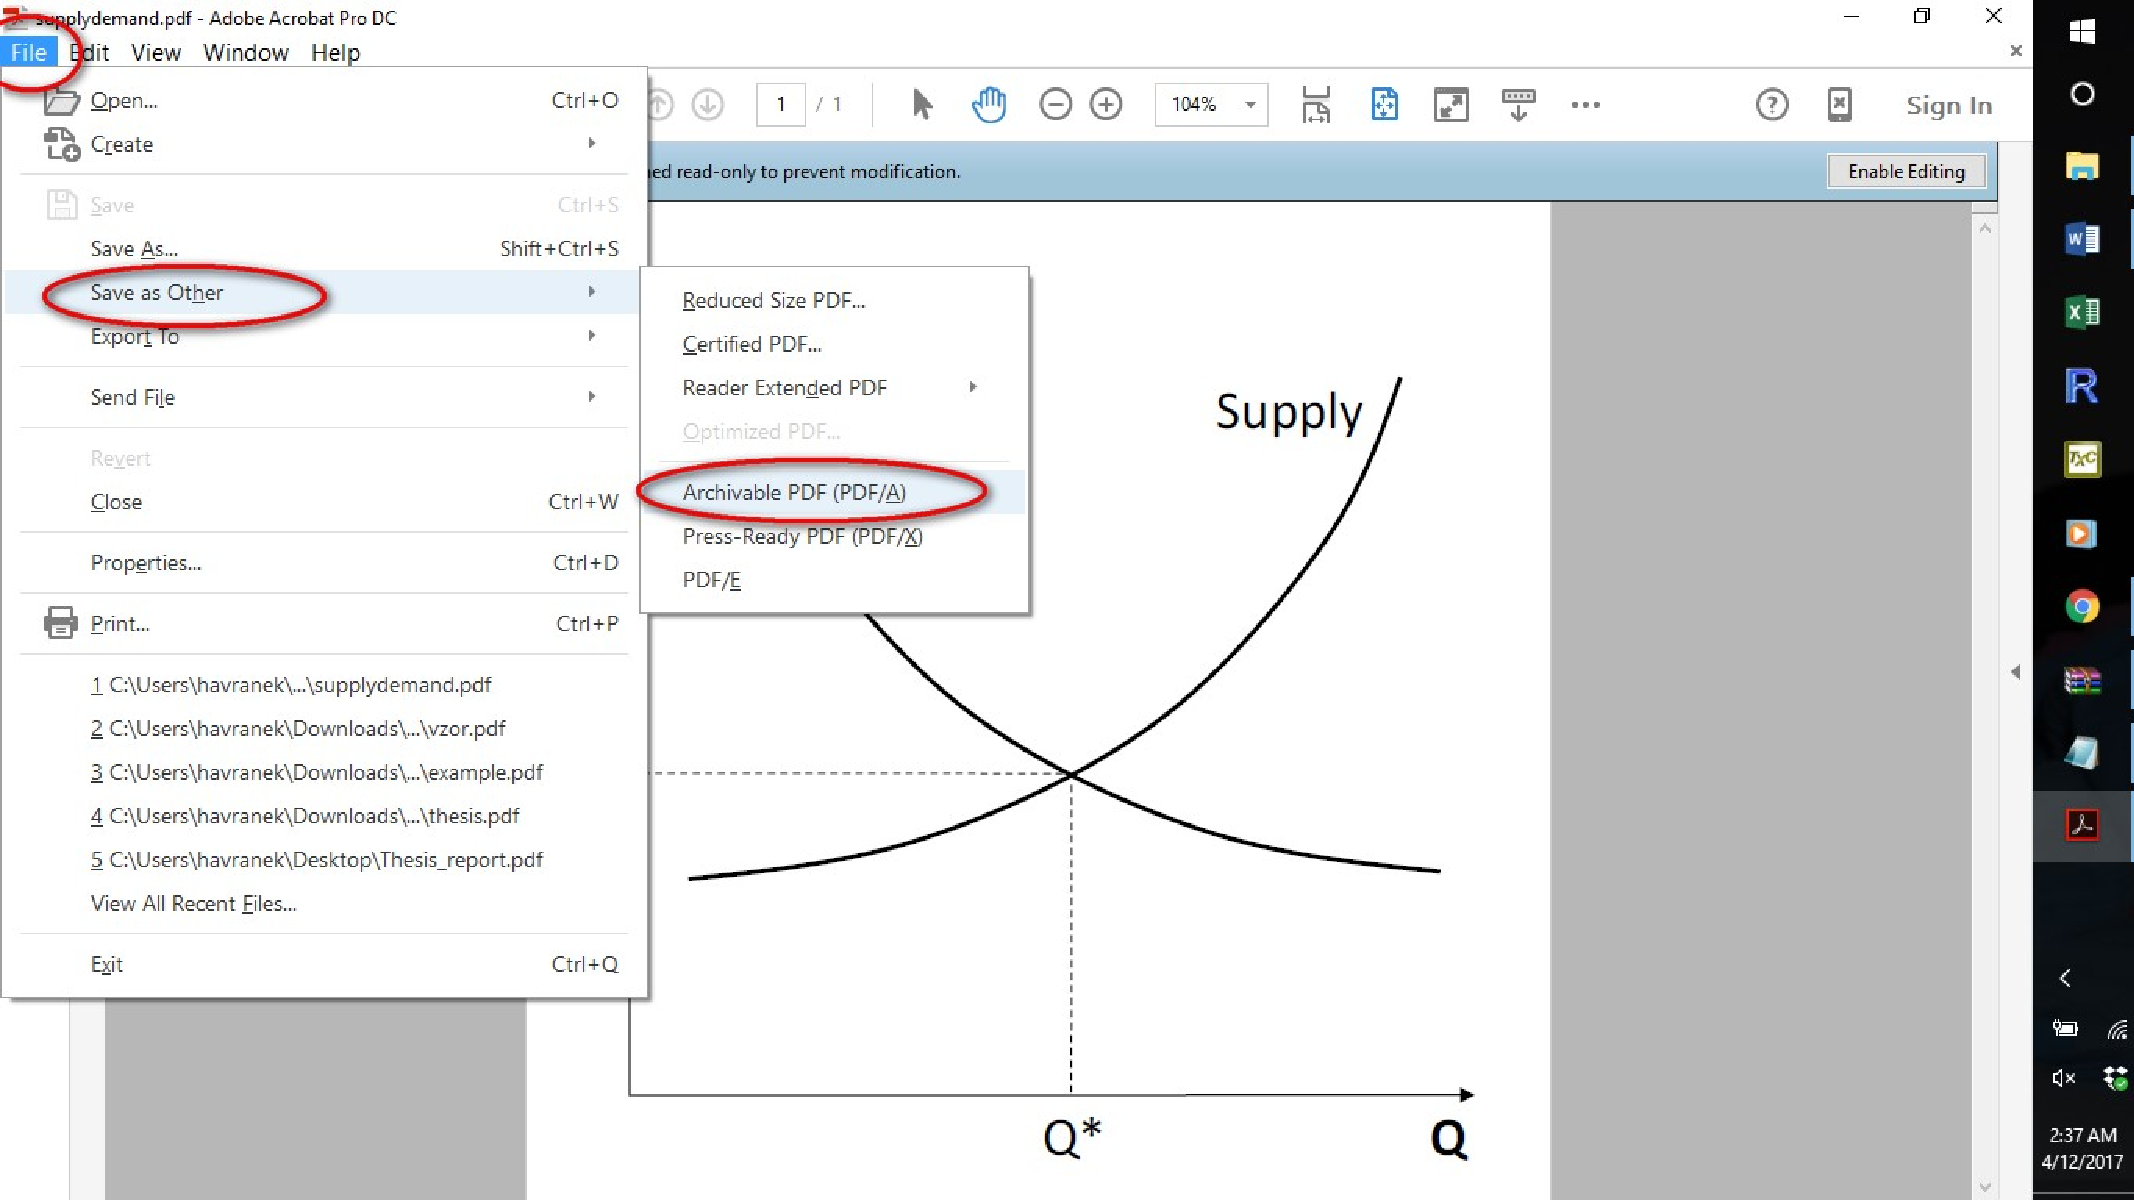
\includegraphics[width=0.6\textwidth]{Figures/conversion1.pdf}
					\label{fig:conversion1}
				\end{figure}
	\item Save as PDF/A-2u:
			\begin{figure}[!h]
				\centering
					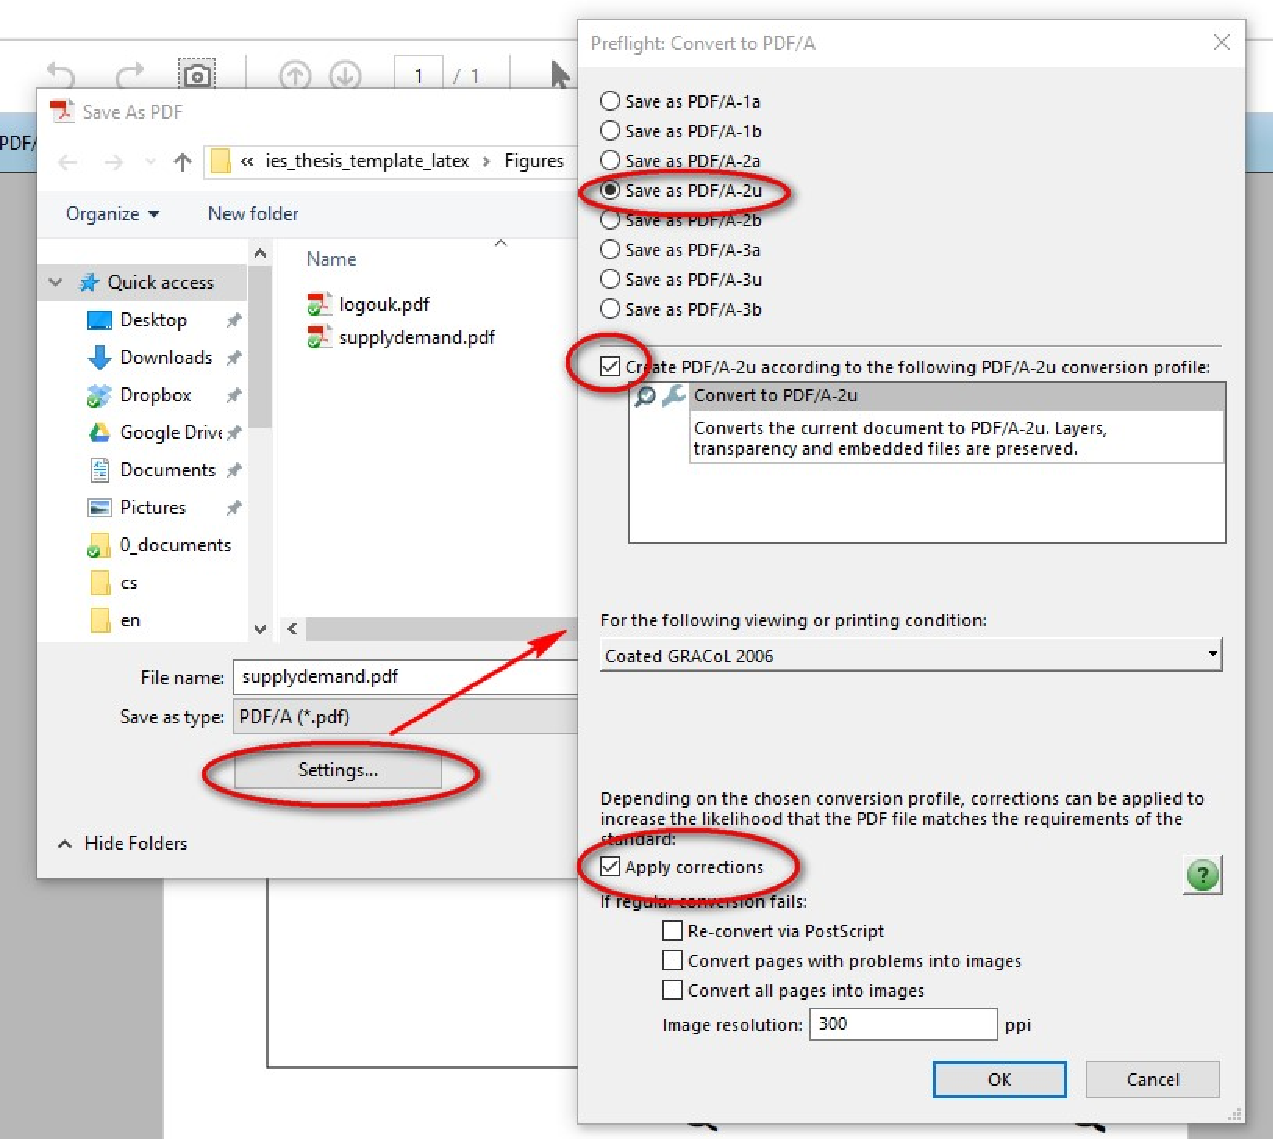
\includegraphics[width=0.6\textwidth]{Figures/conversion2.pdf}
				\label{fig:conversion2}
			\end{figure}
\end{itemize}	


But most of the vector graphics gets distorted to lower quality in Adobe (like pictures in pdfs generated from Stata, unless jpeg is sufficient for you). You can also use GhostScript, the conversion tool is provided by courtesy of the Faculty of Mathematics and Physics at

\vspace{0.5cm}
\textbf{\href{https://kam.mff.cuni.cz/pdfix/}{https://kam.mff.cuni.cz/pdfix/}}
\vspace{0.5cm}

Text text text text text text.\footnote{Text text text text text text text text text text text text text text text. Text text text text text text text text text text. Text text text text text text.} Font of Latin phrases should be consistent: Furthermore, there is no \latinfont{ex post} price effect, all things being equal (\latinfont{ceteris paribus}). This is \latinfont{per se} truth.

\begin{figure}[!htbp]
\begin{center}
\caption{Market equilibrium}
\label{fig:supply}
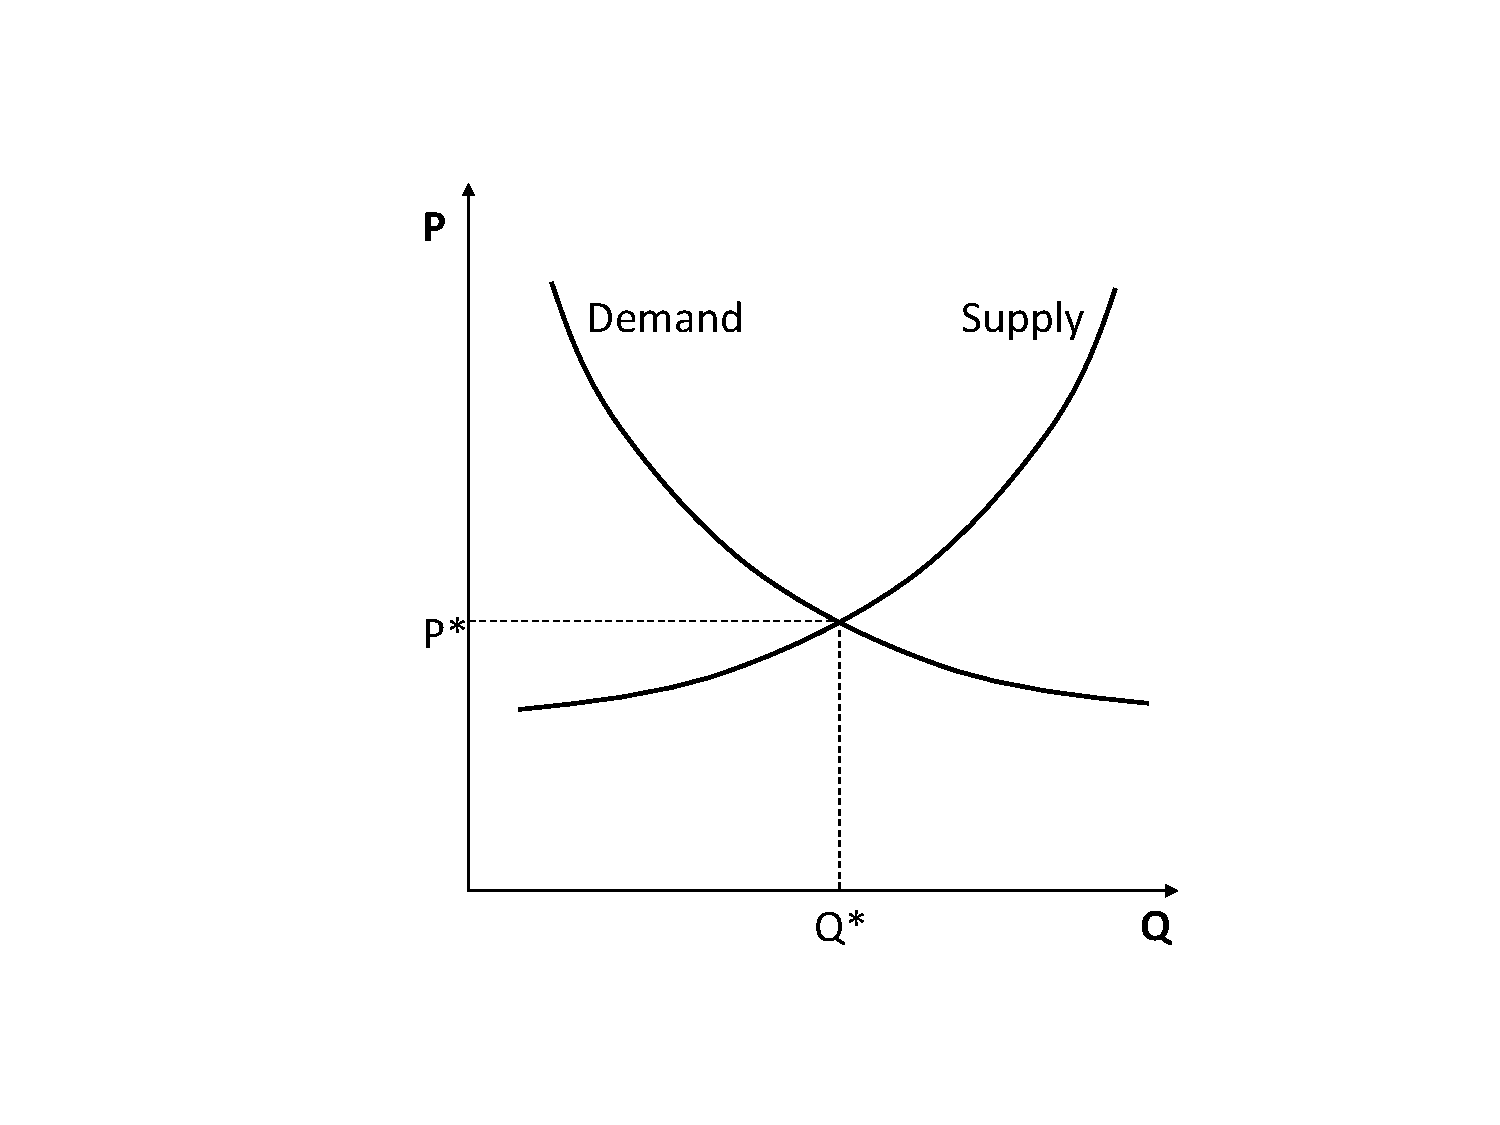
\includegraphics[width=60mm]{Figures/supplydemand}
\end{center}\vspace{-0.5cm}
\begin{source}\cite{Haufler2006}.\end{source}
\end{figure}

Look at the \autoref{fig:supply}. Text text text text text text text text text text. Text text text text text text. Text text text text text text text text text text. Text text text text text text text text text text.



\section{Tables}

If you use Stata, you might want to check the \texttt{sutex}, \texttt{outtable}, \texttt{outtex}, and \texttt{estout} tools, which help you with exporting Stata tables to \LaTeX{}.

\begin{table}[!htbp]
\begin{center}
	\caption[Calibration table]{Model's predictions}\label{tab:values}
\begin{tabular}{lrrrrrrrrrr}
\toprule
\textit{Case} &        $Y_1$ &        $Y_2$ &  $\tau_1$ &  $\tau_2$ &          $a$ &          $n$\\
\midrule
CR---Slovakia &       10.9 &         10 &       0.24 &       0.19 &          1,000 &       2.16\\

CR---Poland &       13.3 &         12 &       0.24 &       0.19 &          1,000 &       0.38\\

CR---Hungary &       10.4 &          8 &       0.24 &       0.16 &          1,000 &        1.10\\
\bottomrule
\end{tabular}  
\end{center}
\begin{source} If the source is author himself (like a calculation output), this line is redundant.\end{source}
\end{table}

Text text text text text text text text text text text text text text text. Text text text text text text text text text text. Text text text text text text. Text text text text text text text text text text. Text text text text text text text text text text.

\section{Boxes}

Text text text text text text text text text text text text text text text. Text text text text text text text text text text. Text text text text text text. Text text text text text text text text text text. Text text text text text text text text text text. Let us make a box:

\begin{figure}[!htbp]
\begin{center}
\caption{Boxy's example}\label{box:values}
\begin{boxeditemize}
	\item Welcome to Boxy paragraph. 
We sincerely hope you will
all enjoy the show.
	\item
Welcome to Boxy paragraph.
We sincerely hope you will
all enjoy the show.
	\item 
Welcome to Boxy paragraph.
We sincerely hope you will
all enjoy the show.
\end{boxeditemize}
\end{center}
\begin{source}\cite{Haaparanta1996}\end{source}
\end{figure}

Text text text text text text text text text text text text text text text. Text text text text text text text text text text. Text text text text text text. Text text text text text text text text text text. Text text text text text text text text text text.

\section{Theorems, Definitions, \ldots}

\begin{defin}[My original definition]\label{de:definice1}
This is a definition.
\end{defin}

\begin{ass}[My realistic assumption]\label{as:predpoklad1}
This is an assumption.
\end{ass}

\begin{prop}[My clever proposition]\label{pr:veta1}
This is a proposition.
\end{prop}

\begin{lemma}[My useful lemma]\label{le:lemma1}
This is a lemma.
\end{lemma}

\begin{exam}\label{ex:priklad1}
This is an example.
\end{exam}

\begin{proof}
This is a proof.
\end{proof}

\section{Equations}
\label{rovnice}

\subsection{Nonumbered Equations}

Text text text text text text text text text text text text text text text. Text text text text text text text text text text. Text text text text text text. Text text text text text text text text text text. Text text text text text text text text text text.

    \[ U = \underbrace{\int_0^{\infty} \frac{1}{1-\sigma}\left(C^{1-\sigma} -1 \right) e^{-\rho t} \ud t}_\text{meaning of life} \]

\subsection{Numbered Equations}

Text text text text text text text text text text text text text text text. Text text text text text text text text text text. Text text text text text text. Text text text text text text text text text text. Text text text text text text text text text text.
\begin{equation}\label{eq:rovnice1}
    U = \int_0^{\infty} \overbrace{ \frac{1}{1-\sigma}\left(C^{1-\sigma} -1 \right)}^\text{instantaneous utility} e^{-\rho t} \ud t
\end{equation}

\subsection{Matrix Equations}

Text text text text text text text text text text text text text text text. Text text text text text text text text text text. Text text text text text text. Text text text text text text text text text text. Text text text text text text text text text text.

\begin{equation}\label{eq:rovnice2}
    \mat{A} = \mat{B} + \mat{C}
\end{equation}

\section{Cross-references}

\begin{itemize}
    \item to literature~\citep[pg.~10]{Bjorvatn2006} 	
            or~\citet[pg.~10]{Haufler2006},
    \item to~\autoref{fig:supply},														%or use \autoref
    \item see~\autoref{tab:values},
    \item to~\autoref{rovnice},
    \item to~\defref{de:definice1}, to~\proref{pr:veta1},
            \exaref{ex:priklad1}, 
    \item to equations like this: see~\eqref{eq:rovnice1}.
\end{itemize}

\section{Source codes}

You can input a source code like this:
\begin{matlab}{.9\linewidth}{dgreen}
    omega = 1;
    syms zeta;
    jmn = [1 2*zeta*omega omega^2];
    figure(1);
        for zeta = 1E-5 : 0.2 : 1+1E-12
            G = tf(omega^2,subs([1 2*zeta*omega omega^2]));
            bode(G); hold on;
        end
    legend('\zeta = 0','\zeta = 0,2','\zeta = 0,4','\zeta = 0,6',');
\end{matlab}
Should you prefer a different font size, redefine file \texttt{Styles/Mystyle.sty}.



\section{Paragraphs}

Usually you should not use the first person singular (I) in your text, write we instead. As a general recommendation, use the first person sparsely, sometimes it can be replaced by a phrase like ``This work presents \ldots.''

Text text text text text text text text text text text text text text text. Text text text text text text text text text text. Text text text text text text. Text text text text text text text text text text. Text text text text text text text text text text. Text text text text text text \citep{Haufler2006}. Let us make two paragraphs:

\paragraph{Proin} Text text text text text text text text text text text text text text text. Text text text text text text text text text text. Text text text text text text. Text text text text text text text text text text. Text text text text text text text text text text.
Text text text text text text text text text text text text text text text. Text text text text text text text text text text. Text text text text text text. And a subparagraph:
\subparagraph{Velit} Text text text text text text text text text text text text text text text. Text text text text text text text text text text. Text text text text text text. Text text text text text text text text text text. Text text text text text text text text text text.



\chapter{Title of Chapter Four}
\label{chap:four}

\section{Title of Section One}

Many people use simple n-dash in many occasions -- like this --, where however typographic convention---it looks a bit strange at first sight---requires m-dash. Text text text text text text text text text text text text text text text. Text text text text text text text text text text. Text text text text text text \citet{Haufler2006}. 

Text text text text text text text text text text text text text text text. Text text text text text text text text text text. Text text text text text text. Text text text text text text text text text text text text text text text. Text text text text text text text text text text. Text text text text text text \citet{Wells2001}. Let us describe the following animals:

\begin{description}
\item[Item 1] Text text text text text text text text text text text text text text text. Text text text text text text text text text text. Text text text text text text. Text text text text text text text text text text text text text text text. Text text text text text text text text text text. Text text text text text text.
\item[Item 2] Text text text text text text text text text text text text text text text. Text text text text text text text text text text. Text text text text text text. Text text text text text text text text text text text text text text text. Text text text text text text text text text text. Text text text text text text.
\end{description}

Text text text text text text text text text text text text text text text. Text text text text text text text text text text. Text text text text text text. Text text text text text text text text text text text text text text text. Text text text text text text text text text text. Text text text text text text. See what Edmund Burke said about the duties of a Member of Parliament (Speech To The Electors Of Bristol At The Conclusion Of The Poll, November 3, 1774):

\begin{quotesmall}
It ought to be the happiness and glory of a representative to live in the strictest union, the closest correspondence, and the most unreserved communication with his constituents. Their wishes ought to have great weight with him; their opinion, high respect; their business, unremitted attention. It is his duty to sacrifice his repose, his pleasures, his satisfactions, to theirs; and above all, ever, and in all cases, to prefer their interest to his own. But his unbiased opinion, his mature judgment, his enlightened conscience, he ought not to sacrifice to you, to any man, or to any set of men living. These he does not derive from your pleasure; no, nor from the law and the constitution. They are a trust from Providence, for the abuse of which he is deeply answerable. Your representative owes you, not his industry only, but his judgment; and he betrays, instead of serving you, if he sacrifices it to your opinion.
\end{quotesmall}

Text text text text text text text text text text text text text text text. Text text text text text text text text text text. Text text text text text text.Text text text text text text text text text text text text text text text. Text text text text text text text text text text. Text text text text text text.

\begin{listi}
	\item The first item, the first item, the first item, the first item, the first item, the first item,
	\item and the second item.
\end{listi}

\begin{lista}
	\item The first item, the first item, the first item, the first item, the first item, the first item, 
	\item and the second item.
\end{lista}

Text text text text text text text text text text text text text text text. Text text text text text text text text text text. Text text text text text text. Text text text text text text text text text text text text text text text. Text text text text text text text text text text. Text text text text text text. Text text text text text text text text text text text text text text text. Text text text text text text text text text text. Text text text text text text \citet{Blomstrom2003}. 
\chapter{Title of Chapter Five}
\label{chap:five}

\section{Title of Section One}

The following checklist should help in avoiding some frequently made mistakes, if any of the following propositions apply for your thesis, there is a problem:

\begin{itemize} 
		\item You have citations in your abstract.
		\item The introduction does not cover the three parts as described in \autoref{chap:one}.
		\item The introduction contains subheadings.
		\item You described different aspects than promised in the title.
		\item You copied some parts of the text from other work without proper referencing and citing.
		\item You used automatic translation tools to produce text by translating it from another language.
		\item Your thesis contains many typos and grammatical errors. (Use an electronic spell checker. Please!)
		\item You used color in your figures and refer to the ``blue'' line (assume that your readers use a monochrome printer).
		\item You mainly used websites and other unrefereed material as your sources or you used Wikipedia as your source.
		\item You refer to something in your conclusion which you have not mentioned before.
		\item Some forenames in the references are abbreviated, some not.
		\item Some references miss a publishing date.
\end{itemize}



\chapter{Useful Hints}
\label{chap:six}

If you write in English, you might find the following hint
useful: The indefinite article a is used as an before a
vowel sound---for example an apple, an hour, an unusual
thing, an \ac{MNC} (because the acronym is pronounced Em-En-See). Before a consonant sound represented
by a vowel letter a is usual---for example a one, a
unique thing, a historic chance. Few more tips to follow:


\begin{itemize}
\item Don't give orders---don't write in the imperative mood---unless you are training to be a teacher.
\item Avoid the use of questions. You may know the answer: does your reader? It's much safer to tell her, or him.
\item Do not become entangled in the problems of `sexist' language. It is much easier to write in the plural. ``Students should check their work'' is good English. ``A student should check---'' is also good English, but now the problems begin: ``---her work?'' ``---his work?'' Which? You can write ``his or her,'' but that seems clumsy. Stick to the plural.
\item If you must refer to yourself, use the third person such as ``The present writer would recommend that \ldots'' may be useful.
\item Use the full forms of words and phrases, not contractions like ``he's,'' ``don't,'' etc. Keep the apostrophe to indicate possession---and use it correctly. Academics really sneer at students who use the ``Greengrocer's apostrophe.''
\end{itemize}


\begin{itemize}
\item Do not despise short, workmanlike, and effective plain English words. If they mean what you want to say. Accurately.
\item Avoid the use of humor in academic writing---unless you are very sure of yourself.
\item Even when you are not being funny, avoid the use of irony or sarcasm.
\item Paragraphs in academic English should contain more than one sentence. (Short paragraphs look as if you are writing for a tabloid newspaper---or a simple Template!) I guess that the average academic book runs to two or three paragraphs per page. Look at the books in your subject, and get a feel for how long your own paragraphs should be when you are imitating the academic style.
\item Use the word that more in formal writing than most of us do in speech---particularly after such verbs of utterance as to say, to report, to think etc. It can help to make your writing much clearer.
\item Develop an academic vocabulary. The `long words' you learn in the course of your studies are long usually because they have more precise meanings than their less formal equivalents. They are therefore better when you want to be accurate. (Also they allow you to sound like someone who deserves a degree.)
\end{itemize}



\begin{itemize}
\item  Use as few words as you can; but use enough words to express your meaning as fully as you can. Your judgment of what is appropriate here is part of what you should learn throughout your course.
\item  Avoid lazy words such as ``nice''. It is usually better to say ``acquire'' or ``obtain'' than ``get;'' and it may be better, if you mean ``through the use of money,'' to say ``purchase'' or---better still---''buy.''
\item A short word like ``buy'' is better than a long one like ``purchase''---unless the long one is more accurate. A ``statutory instrument'' is better than a ``rule''---to a lawyer, at any rate.
\item Proof-read with care. Ask someone else to help---you may be too close to your work to be able to see your mistakes.
\item If in doubt, choose the more formal, or possibly just the more old-fashioned, of two words. For example, say quotation rather than quote whenever you mean the use of somebody else's words.
\end{itemize}



\begin{itemize}
\item You will often sound more academic if you include doubts in your work---and qualifications. Within the scope of this thesis, the current writer cannot hope to cover all the possible implications of the question.ԍ
\item In this context, the use of litotes sounds very academic. This is the construction where a writer uses a negative with a negative adjective, e.g.\ it is not unlikely that \ldots This does not mean the same as it is probable that \ldots It has a shade of meaning and qualification that can be useful to academic writers.
\end{itemize}





\chapter{Conclusion}
\label{conclusion}

The conclusion should briefly summarize the problem statement and the general content of the work and the emphasize on the main contribution of the work.

When writing the conclusion keep in mind that some readers may not have gone through the whole thesis, but have jumped directly to the conclusion after having read the abstract in order the decide on the personal relevance of the thesis. Therefore, the conclusion should be self contained, which means that a reader should be able to understand the essence of the conclusion without having to read the whole thesis.

The conclusion typically ends with an outlook that describes possible extensions of the presented approaches and of planned future work.

\clearpage
%-----<<< -------- >>>-----

%-----<<< REFERENCES >>>-----
\fancyhead[LO]{\sffamily Bibliography}					%headers in sans serif and not in uppercase
\bibliographystyle{Styles/Stylebib}							%style of literature, you can use e.g. newapa	instead of Styles/Stylebib
\bibliography{Styles/Bibliography}							%bibliography database
\addcontentsline{toc}{chapter}{Bibliography} 		%Add bibliography to the table of contents
\clearpage
%-----<<< ---------- >>>-----

%-----<<< APPENDIXES >>>-----
\backmatter																			%uppercase roman pagination for back matter; appendices start
\autohdr																				%automatic headers     				
\chapter{Additional Data Descriptives}
\label{chap:additional_figures} 

This Appendix gives additional descriptive statistics of the distributions of the predictors. Histograms of all feature distributions is given in Figure \ref{fig:histograms}. The same distributions are also summarized numerically in Table \ref{tab:descriptives}. The numerical values of the correlation matrix of the features is available in \ref{tab:correlation_matrix}.
 
\begin{center}
	\begin{sidewaysfigure}
		\includegraphics[width=\textwidth,height=\textheight,keepaspectratio]{Figures/histograms.pdf}
		\caption{Histograms of All Features}
		\label{fig:histograms}
		\medskip
		\small
		The figure shows how the values of observations are distributed within each feature. The horizontal axis shows the values of the features (which range between $-1$ and $1$), and the vertical axis shows number of observations (or examples in ML terminology) within each bin, in thousands.  
	\end{sidewaysfigure}
\end{center}  
 
\begin{table}
	\resizebox{\textwidth}{!}{\begin{tabular}{lrrrrrrr}
\toprule
{} &  Mean &     Std &     Min &     25\% &     50\% &     75\% &     Max \\
\midrule
52-Week High                               &   0.0 &  0.3071 & -1.0000 & -0.1126 &  0.0765 &  0.1971 &  0.5366 \\
Short-Term Reversal                        &  -0.0 &  0.3704 & -1.0000 & -0.2174 & -0.0023 &  0.2225 &  0.8637 \\
Idiosyncratic Risk                         &   0.0 &  0.4403 & -0.9752 & -0.3038 & -0.0835 &  0.2437 &  1.0000 \\
Volume / Market Value of Equity            &  -0.0 &  0.3747 & -0.4584 & -0.2709 & -0.1219 &  0.1537 &  1.0000 \\
Coefficient of Variation of Share Turnover &   0.0 &  0.4436 & -0.8373 & -0.2992 & -0.0924 &  0.2506 &  1.0000 \\
Max                                        &  -0.0 &  0.4146 & -0.7492 & -0.2925 & -0.0982 &  0.2085 &  1.0000 \\
Whited-Wu Index                            &   0.0 &  0.5424 & -1.0000 & -0.4148 & -0.1142 &  0.4541 &  1.0000 \\
Coskewness                                 &   0.0 &  0.4030 & -1.0000 & -0.2443 &  0.0486 &  0.2453 &  0.8649 \\
Operating Profits to Assets                &   0.0 &  0.3769 & -1.0000 & -0.2765 & -0.1101 &  0.2248 &  1.0000 \\
Lagged Momentum                            &   0.0 &  0.4027 & -1.0000 & -0.2511 & -0.0200 &  0.2385 &  1.0000 \\
Liquidity Beta 5                           &  -0.0 &  0.5324 & -1.0000 & -0.3462 & -0.0257 &  0.3874 &  1.0000 \\
RD / Market Equity                         &  -0.0 &  0.3173 & -0.1806 & -0.1693 & -0.1285 & -0.0438 &  1.0000 \\
Seasonality 6-10 A                         &   0.0 &  0.3523 & -1.0000 & -0.1447 & -0.0287 &  0.1860 &  0.8851 \\
Seasonality 11-15 N                        &  -0.0 &  0.3759 & -1.0000 & -0.2122 & -0.0921 &  0.2069 &  1.0000 \\
Seasonality 2-5 N                          &   0.0 &  0.3515 & -1.0000 & -0.2002 & -0.0198 &  0.2066 &  0.8949 \\
Momentum-Reversal                          &   0.0 &  0.4057 & -1.0000 & -0.2458 & -0.0211 &  0.2385 &  1.0000 \\
Amihud's Measure (Illiquidity)             &  -0.0 &  0.2697 & -0.1343 & -0.1042 & -0.0923 & -0.0689 &  1.0000 \\
Net Operating Assets                       &   0.0 &  0.5027 & -1.0000 & -0.4207 &  0.0598 &  0.3546 &  1.0000 \\
Seasonality 6-10 N                         &   0.0 &  0.3689 & -1.0000 & -0.2252 & -0.0502 &  0.2213 &  1.0000 \\
Seasonality                                &  -0.0 &  0.3361 & -1.0000 & -0.1740 & -0.0120 &  0.1990 &  0.7349 \\
Seasonality 2-5 A                          &  -0.0 &  0.3671 & -1.0000 & -0.2022 & -0.0122 &  0.2224 &  0.8339 \\
Accruals                                   &   0.0 &  0.2727 & -1.0000 & -0.1180 &  0.0590 &  0.1406 &  0.5606 \\
Duration of Equity                         &   0.0 &  0.2035 & -1.0000 & -0.0673 &  0.0419 &  0.1293 &  0.3104 \\
Change in Common Equity                    &  -0.0 &  0.3025 & -1.0000 & -0.1405 & -0.0406 &  0.0960 &  1.0000 \\
Profit Margin                              &  -0.0 &  0.1888 & -1.0000 & -0.0138 &  0.0150 &  0.0378 &  1.0000 \\
Liquidity Beta 3                           &  -0.0 &  0.3286 & -1.0000 & -0.1563 &  0.0863 &  0.1952 &  0.6684 \\
Liquidity Shocks                           &  -0.0 &  0.1244 & -1.0000 &  0.0158 &  0.0201 &  0.0229 &  0.3647 \\
Leverage Component of Book/Price           &   0.0 &  0.1766 & -1.0000 & -0.0197 &  0.0064 &  0.0499 &  0.6213 \\
Earnings Predictability                    &  -0.0 &  0.2439 & -0.0900 & -0.0752 & -0.0701 & -0.0608 &  1.0000 \\
Earnings Forecast-to-Price                 &   0.0 &  0.3024 & -1.0000 & -0.1921 & -0.0080 &  0.1614 &  1.0000 \\
\bottomrule
\end{tabular}
}
	\caption{Descriptive Statistics of the Features}
	\label{tab:descriptives}
\end{table} 
 
\begin{sidewaystable}
	\begin{adjustbox}{scale=0.4,center}
		\begin{tabular}{lrrrrrrrrrrrrrrrrrrrrrrrrrrrrrr}
\toprule
\rot{{} }&\rot{  52-Week High }&\rot{  Short-Term Reversal }&\rot{  Idiosyncratic Risk }&\rot{  Volume / Market Value of Equity }&\rot{  Coefficient of Variation of Share Turnover }&\rot{  Maximum Return }&\rot{  Whited-Wu Index }&\rot{  Coskewness }&\rot{  Operating Profits to Assets }&\rot{  Lagged Momentum }&\rot{  Liquidity Beta 5 }&\rot{  RD / Market Equity }&\rot{  Seasonality 6-10 A }&\rot{  Seasonality 11-15 N }&\rot{  Seasonality 2-5 N }&\rot{  Momentum-Reversal }&\rot{  Amihud's Measure (Illiquidity) }&\rot{  Net Operating Assets }&\rot{  Seasonality 6-10 N }&\rot{  Seasonality }&\rot{  Seasonality 2-5 A }&\rot{  Accruals }&\rot{  Duration of Equity }&\rot{  Change in Common Equity }&\rot{  Profit Margin }&\rot{  Liquidity Beta 3 }&\rot{  Liquidity Shocks }&\rot{  Leverage Component of Book/Price }&\rot{  Earnings Predictability }&\rot{  Earnings Forecast-to-Price }\\
\midrule
52-Week High                               &         1.000 &                0.382 &              -0.345 &                           -0.340 &                                      -0.056 &          -0.224 &           -0.004 &      -0.031 &                       -0.001 &            0.178 &            -0.144 &              -0.059 &              -0.007 &                0.014 &             -0.119 &             -0.060 &                          -0.067 &                -0.038 &              -0.037 &       -0.021 &             -0.017 &    -0.052 &               0.182 &                   -0.073 &          0.064 &             0.055 &            -0.117 &                            -0.060 &                    0.026 &                       0.004 \\
Short-Term Reversal                        &         0.382 &                1.000 &               0.105 &                           -0.093 &                                       0.025 &           0.304 &            0.019 &       0.001 &                       -0.003 &            0.013 &            -0.006 &              -0.027 &               0.017 &               -0.006 &             -0.011 &             -0.018 &                           0.041 &                -0.010 &              -0.020 &        0.017 &              0.003 &    -0.006 &               0.070 &                   -0.002 &         -0.000 &            -0.010 &            -0.100 &                            -0.014 &                    0.004 &                      -0.066 \\
Idiosyncratic Risk                         &        -0.345 &                0.105 &               1.000 &                            0.230 &                                       0.189 &           0.817 &            0.093 &       0.022 &                        0.021 &            0.055 &             0.094 &              -0.013 &              -0.000 &               -0.060 &              0.087 &              0.030 &                           0.224 &                 0.029 &              -0.012 &        0.038 &              0.013 &     0.045 &              -0.020 &                    0.109 &         -0.090 &            -0.057 &            -0.099 &                             0.043 &                   -0.036 &                      -0.114 \\
Volume / Market Value of Equity            &        -0.340 &               -0.093 &               0.230 &                            1.000 &                                       0.095 &           0.178 &           -0.015 &       0.022 &                        0.045 &            0.062 &             0.301 &               0.091 &               0.003 &               -0.014 &              0.105 &              0.073 &                          -0.019 &                 0.030 &               0.019 &        0.035 &              0.013 &    -0.014 &              -0.098 &                    0.051 &         -0.058 &            -0.211 &            -0.000 &                             0.037 &                    0.016 &                       0.064 \\
Coefficient of Variation of Share Turnover &        -0.056 &                0.025 &               0.189 &                            0.095 &                                       1.000 &           0.137 &            0.100 &      -0.002 &                       -0.009 &            0.045 &             0.018 &              -0.082 &              -0.012 &               -0.059 &              0.037 &              0.015 &                           0.405 &                 0.053 &              -0.025 &        0.012 &              0.000 &     0.039 &              -0.000 &                    0.094 &          0.014 &            -0.007 &            -0.140 &                             0.013 &                   -0.044 &                      -0.005 \\
Maximum Return                             &        -0.224 &                0.304 &               0.817 &                            0.178 &                                       0.137 &           1.000 &            0.060 &       0.026 &                        0.002 &            0.038 &             0.114 &              -0.004 &               0.008 &               -0.039 &              0.062 &              0.013 &                           0.171 &                 0.010 &              -0.009 &        0.029 &              0.008 &     0.040 &              -0.007 &                    0.076 &         -0.080 &            -0.077 &            -0.091 &                             0.022 &                   -0.028 &                      -0.114 \\
Whited-Wu Index                            &        -0.004 &                0.019 &               0.093 &                           -0.015 &                                       0.100 &           0.060 &            1.000 &       0.001 &                       -0.203 &            0.057 &            -0.158 &              -0.226 &              -0.030 &               -0.126 &              0.057 &              0.044 &                           0.129 &                -0.313 &              -0.075 &        0.006 &              0.001 &     0.134 &              -0.065 &                   -0.028 &         -0.070 &             0.034 &            -0.049 &                             0.039 &                   -0.049 &                      -0.090 \\
Coskewness                                 &        -0.031 &                0.001 &               0.022 &                            0.022 &                                      -0.002 &           0.026 &            0.001 &       1.000 &                       -0.020 &           -0.018 &             0.139 &              -0.029 &              -0.017 &               -0.014 &             -0.006 &             -0.030 &                          -0.011 &                -0.032 &              -0.056 &       -0.001 &             -0.002 &     0.030 &              -0.004 &                   -0.001 &         -0.005 &             0.038 &             0.005 &                            -0.017 &                   -0.020 &                      -0.060 \\
Operating Profits to Assets                &        -0.001 &               -0.003 &               0.021 &                            0.045 &                                      -0.009 &           0.002 &           -0.203 &      -0.020 &                        1.000 &           -0.007 &            -0.045 &               0.243 &               0.016 &                0.034 &              0.097 &              0.018 &                          -0.023 &                 0.150 &               0.050 &        0.033 &              0.031 &    -0.110 &               0.229 &                    0.108 &          0.184 &             0.069 &             0.011 &                             0.013 &                    0.010 &                       0.004 \\
Lagged Momentum                            &         0.178 &                0.013 &               0.055 &                            0.062 &                                       0.045 &           0.038 &            0.057 &      -0.018 &                       -0.007 &            1.000 &             0.037 &              -0.058 &              -0.007 &               -0.040 &              0.007 &             -0.004 &                           0.105 &                -0.003 &              -0.029 &        0.150 &             -0.029 &    -0.018 &               0.126 &                    0.043 &         -0.009 &            -0.072 &            -0.136 &                            -0.014 &                    0.001 &                      -0.001 \\
Liquidity Beta 5                           &        -0.144 &               -0.006 &               0.094 &                            0.301 &                                       0.018 &           0.114 &           -0.158 &       0.139 &                       -0.045 &            0.037 &             1.000 &               0.054 &               0.041 &                0.115 &              0.072 &              0.030 &                          -0.006 &                 0.072 &               0.131 &        0.039 &              0.036 &    -0.008 &              -0.042 &                   -0.051 &         -0.034 &            -0.512 &            -0.017 &                            -0.018 &                    0.013 &                       0.049 \\
RD / Market Equity                         &        -0.059 &               -0.027 &              -0.013 &                            0.091 &                                      -0.082 &          -0.004 &           -0.226 &      -0.029 &                        0.243 &           -0.058 &             0.054 &               1.000 &              -0.006 &                0.037 &             -0.098 &             -0.051 &                          -0.070 &                 0.032 &              -0.026 &       -0.030 &             -0.025 &    -0.096 &              -0.072 &                   -0.070 &         -0.128 &            -0.060 &             0.042 &                             0.024 &                    0.042 &                      -0.039 \\
Seasonality 6-10 A                         &        -0.007 &                0.017 &              -0.000 &                            0.003 &                                      -0.012 &           0.008 &           -0.030 &      -0.017 &                        0.016 &           -0.007 &             0.041 &              -0.006 &               1.000 &                0.017 &             -0.030 &             -0.017 &                          -0.015 &                 0.026 &               0.018 &        0.403 &              0.015 &    -0.007 &               0.026 &                   -0.008 &          0.014 &            -0.014 &             0.007 &                            -0.005 &                    0.016 &                       0.002 \\
Seasonality 11-15 N                        &         0.014 &               -0.006 &              -0.060 &                           -0.014 &                                      -0.059 &          -0.039 &           -0.126 &      -0.014 &                        0.034 &           -0.040 &             0.115 &               0.037 &               0.017 &                1.000 &             -0.066 &             -0.040 &                          -0.064 &                 0.048 &               0.048 &       -0.035 &             -0.016 &    -0.024 &               0.042 &                   -0.066 &         -0.013 &            -0.011 &             0.021 &                            -0.022 &                    0.034 &                       0.005 \\
Seasonality 2-5 N                          &        -0.119 &               -0.011 &               0.087 &                            0.105 &                                       0.037 &           0.062 &            0.057 &      -0.006 &                        0.097 &            0.007 &             0.072 &              -0.098 &              -0.030 &               -0.066 &              1.000 &              0.370 &                           0.051 &                 0.081 &              -0.053 &        0.009 &             -0.013 &     0.045 &               0.150 &                    0.242 &          0.090 &            -0.069 &            -0.005 &                             0.018 &                    0.006 &                       0.058 \\
Momentum-Reversal                          &        -0.060 &               -0.018 &               0.030 &                            0.073 &                                       0.015 &           0.013 &            0.044 &      -0.030 &                        0.018 &           -0.004 &             0.030 &              -0.051 &              -0.017 &               -0.040 &              0.370 &              1.000 &                           0.026 &                 0.014 &              -0.018 &        0.011 &              0.024 &    -0.010 &               0.100 &                    0.099 &          0.030 &            -0.065 &            -0.001 &                            -0.003 &                    0.005 &                       0.039 \\
Amihud's Measure (Illiquidity)             &        -0.067 &                0.041 &               0.224 &                           -0.019 &                                       0.405 &           0.171 &            0.129 &      -0.011 &                       -0.023 &            0.105 &            -0.006 &              -0.070 &              -0.015 &               -0.064 &              0.051 &              0.026 &                           1.000 &                 0.051 &              -0.021 &        0.013 &              0.003 &     0.033 &              -0.022 &                    0.106 &         -0.050 &             0.023 &            -0.494 &                             0.044 &                   -0.041 &                      -0.013 \\
Net Operating Assets                       &        -0.038 &               -0.010 &               0.029 &                            0.030 &                                       0.053 &           0.010 &           -0.313 &      -0.032 &                        0.150 &           -0.003 &             0.072 &               0.032 &               0.026 &                0.048 &              0.081 &              0.014 &                           0.051 &                 1.000 &               0.092 &        0.030 &              0.032 &    -0.013 &               0.059 &                    0.353 &          0.160 &             0.011 &            -0.015 &                            -0.151 &                   -0.017 &                       0.046 \\
Seasonality 6-10 N                         &        -0.037 &               -0.020 &              -0.012 &                            0.019 &                                      -0.025 &          -0.009 &           -0.075 &      -0.056 &                        0.050 &           -0.029 &             0.131 &              -0.026 &               0.018 &                0.048 &             -0.053 &             -0.018 &                          -0.021 &                 0.092 &               1.000 &       -0.030 &             -0.009 &    -0.015 &               0.085 &                    0.007 &          0.044 &            -0.049 &             0.014 &                            -0.015 &                    0.027 &                       0.011 \\
Seasonality                                &        -0.021 &                0.017 &               0.038 &                            0.035 &                                       0.012 &           0.029 &            0.006 &      -0.001 &                        0.033 &            0.150 &             0.039 &              -0.030 &               0.403 &               -0.035 &              0.009 &              0.011 &                           0.013 &                 0.030 &              -0.030 &        1.000 &              0.555 &     0.009 &               0.058 &                    0.060 &          0.029 &            -0.019 &            -0.016 &                             0.003 &                   -0.001 &                      -0.002 \\
Seasonality 2-5 A                          &        -0.017 &                0.003 &               0.013 &                            0.013 &                                       0.000 &           0.008 &            0.001 &      -0.002 &                        0.031 &           -0.029 &             0.036 &              -0.025 &               0.015 &               -0.016 &             -0.013 &              0.024 &                           0.003 &                 0.032 &              -0.009 &        0.555 &              1.000 &     0.012 &               0.044 &                    0.056 &          0.035 &            -0.022 &            -0.004 &                             0.004 &                    0.002 &                       0.012 \\
Accruals                                   &        -0.052 &               -0.006 &               0.045 &                           -0.014 &                                       0.039 &           0.040 &            0.134 &       0.030 &                       -0.110 &           -0.018 &            -0.008 &              -0.096 &              -0.007 &               -0.024 &              0.045 &             -0.010 &                           0.033 &                -0.013 &              -0.015 &        0.009 &              0.012 &     1.000 &              -0.075 &                    0.102 &          0.028 &             0.028 &             0.006 &                            -0.004 &                   -0.033 &                       0.013 \\
Duration of Equity                         &         0.182 &                0.070 &              -0.020 &                           -0.098 &                                      -0.000 &          -0.007 &           -0.065 &      -0.004 &                        0.229 &            0.126 &            -0.042 &              -0.072 &               0.026 &                0.042 &              0.150 &              0.100 &                          -0.022 &                 0.059 &               0.085 &        0.058 &              0.044 &    -0.075 &               1.000 &                    0.044 &          0.010 &             0.049 &            -0.055 &                            -0.367 &                    0.019 &                      -0.178 \\
Change in Common Equity                    &        -0.073 &               -0.002 &               0.109 &                            0.051 &                                       0.094 &           0.076 &           -0.028 &      -0.001 &                        0.108 &            0.043 &            -0.051 &              -0.070 &              -0.008 &               -0.066 &              0.242 &              0.099 &                           0.106 &                 0.353 &               0.007 &        0.060 &              0.056 &     0.102 &               0.044 &                    1.000 &          0.135 &             0.022 &            -0.037 &                             0.091 &                   -0.017 &                       0.019 \\
Profit Margin                              &         0.064 &               -0.000 &              -0.090 &                           -0.058 &                                       0.014 &          -0.080 &           -0.070 &      -0.005 &                        0.184 &           -0.009 &            -0.034 &              -0.128 &               0.014 &               -0.013 &              0.090 &              0.030 &                          -0.050 &                 0.160 &               0.044 &        0.029 &              0.035 &     0.028 &               0.010 &                    0.135 &          1.000 &             0.049 &             0.039 &                             0.038 &                   -0.005 &                       0.217 \\
Liquidity Beta 3                           &         0.055 &               -0.010 &              -0.057 &                           -0.211 &                                      -0.007 &          -0.077 &            0.034 &       0.038 &                        0.069 &           -0.072 &            -0.512 &              -0.060 &              -0.014 &               -0.011 &             -0.069 &             -0.065 &                           0.023 &                 0.011 &              -0.049 &       -0.019 &             -0.022 &     0.028 &               0.049 &                    0.022 &          0.049 &             1.000 &             0.003 &                            -0.008 &                   -0.037 &                      -0.080 \\
Liquidity Shocks                           &        -0.117 &               -0.100 &              -0.099 &                           -0.000 &                                      -0.140 &          -0.091 &           -0.049 &       0.005 &                        0.011 &           -0.136 &            -0.017 &               0.042 &               0.007 &                0.021 &             -0.005 &             -0.001 &                          -0.494 &                -0.015 &               0.014 &       -0.016 &             -0.004 &     0.006 &              -0.055 &                   -0.037 &          0.039 &             0.003 &             1.000 &                             0.003 &                    0.012 &                       0.037 \\
Leverage Component of Book/Price           &        -0.060 &               -0.014 &               0.043 &                            0.037 &                                       0.013 &           0.022 &            0.039 &      -0.017 &                        0.013 &           -0.014 &            -0.018 &               0.024 &              -0.005 &               -0.022 &              0.018 &             -0.003 &                           0.044 &                -0.151 &              -0.015 &        0.003 &              0.004 &    -0.004 &              -0.367 &                    0.091 &          0.038 &            -0.008 &             0.003 &                             1.000 &                   -0.008 &                       0.047 \\
Earnings Predictability                    &         0.026 &                0.004 &              -0.036 &                            0.016 &                                      -0.044 &          -0.028 &           -0.049 &      -0.020 &                        0.010 &            0.001 &             0.013 &               0.042 &               0.016 &                0.034 &              0.006 &              0.005 &                          -0.041 &                -0.017 &               0.027 &       -0.001 &              0.002 &    -0.033 &               0.019 &                   -0.017 &         -0.005 &            -0.037 &             0.012 &                            -0.008 &                    1.000 &                       0.020 \\
Earnings Forecast-to-Price                 &         0.004 &               -0.066 &              -0.114 &                            0.064 &                                      -0.005 &          -0.114 &           -0.090 &      -0.060 &                        0.004 &           -0.001 &             0.049 &              -0.039 &               0.002 &                0.005 &              0.058 &              0.039 &                          -0.013 &                 0.046 &               0.011 &       -0.002 &              0.012 &     0.013 &              -0.178 &                    0.019 &          0.217 &            -0.080 &             0.037 &                             0.047 &                    0.020 &                       1.000 \\
\bottomrule
\end{tabular}

	\end{adjustbox}
	\caption{Features Correlation Matrix}
	\label{tab:correlation_matrix}
	\medspace
	\small
	The matrix shows pairwise correlation coefficients of all features. A visual version of this matrix is available in the main text in Figure \ref{fig:correlation_matrix}.
\end{sidewaystable}



           			%input file
\chapter{Content of Enclosed DVD}

This is optional: you may enclose a DVD to this thesis which contains empirical data and MatLab/R/Stata source codes. Even better so, you can create a special website for your project. Stating in your thesis that the data and source codes are available upon request is enough but please, have them prepared for such requests.

\begin{itemize}
    \item Folder 1: Source codes
    \item Folder 2: Empirical data
\end{itemize}
           			%input file
\clearpage
%-----<<< --------- >>>-----


\end{document}
%-----<<<<<<<<< END OF DOCUMENT >>>>>>>>>-----
